% $Id: paper.tex 253 2008-08-23 05:23:14Z johnmc $

\documentclass[12pt]{article}

% ***************************************************************************
% Standard packages
% ***************************************************************************

\usepackage{cite}
\usepackage{fullpage}

%\usepackage[breaklinks=true]{hyperref} %bookmarksopen,bookmarksnumbered

% NOTE: With approval from Wiley, I changed cpeauth to use [pdftex]{graphicx}
\usepackage{ifpdf}
\ifpdf
  \usepackage[pdftex]{graphicx}
  \usepackage{epstopdf}
\else
  \usepackage[dvips]{graphicx}
  %\usepackage{breakurl} % fix hyperref
\fi

% Not necessary now
%\usepackage{floatflt} % wrapfig seems to be inferior

%\usepackage{hyperref} % bookmarksopen,bookmarksnumbered
%\usepackage{url}

\usepackage{verbatim} % for comment environment

% ***************************************************************************
% Customizations
% ***************************************************************************
% A sane version of verb/texttt (requires url package)
\newcommand{\mytt}{\begingroup \urlstyle{tt}\Url}

% Because the retarded tabbing environment limits you to about 12 tabs
\newcommand{\TB}{\hspace{.20in}}

\newcommand{\figuretextsize}{scriptsize}

% ----------------------------------------------------------
% my common text commands
% ----------------------------------------------------------

\newcommand{\ie}{\emph{i.e.}}  % followed by a comma
\newcommand{\eg}{\emph{e.g.}}  % followed by a comma
\newcommand{\cf}{\emph{cf.}}   % always followed by a space
\newcommand{\Cf}{\emph{Cf.}}   % always followed by a space
\newcommand{\etc}{\emph{etc.}}  % 
\newcommand{\etal}{\emph{et al.}}
\newcommand{\viceversa}{\emph{vice versa}}
\newcommand{\naive}{na\"{i}ve}
\newcommand{\nee}{ne\'{e}} 


% ----------------------------------------------------------
% tools
% ----------------------------------------------------------

\newcommand{\HPCToolkit}{\textsc{HPCToolkit}}
\newcommand{\hpcrun}{\texttt{hpcrun}}
\newcommand{\hpcstruct}{\texttt{hpcstruct}}
\newcommand{\hpcprof}{\texttt{hpcprof}}
\newcommand{\hpcviewer}{\texttt{hpcviewer}}
\newcommand{\hpctraceview}{\texttt{hpctraceview}}

\newcommand{\gprof}{\texttt{gprof}}

\newcommand{\binutils}{\texttt{binutils}}

\newcommand{\Unix}{\textsc{Unix}}

% ----------------------------------------------------------
% codes
% ----------------------------------------------------------

\newcommand{\hmc}{\texttt{hmc}}

% ***************************************************************************
% Document
% ***************************************************************************

\begin{document}

% ---------------------------------------------------------------------------
% ---------------------------------------------------------------------------

% Page limit: 15 pages
% Due date: Aug 15 (was July 31st)



\title{Effective Strategies for Analyzing Program Performance with \HPCToolkit{}}

\author{The \HPCToolkit{} Project Team}

\maketitle



\begin{abstract}
\HPCToolkit{} is an integrated suite of tools that supports measurement, analysis, attribution, and presentation of application performance for both sequential and parallel programs. Here we describe some proven strategies for using measurement data to identify performance bottlenecks in both serial and parallel codes.
\end{abstract}


\section{Computing derived metrics}

Modern computer systems  provide access to a rich set of hardware 
performance counters that can directly measure various aspects of a program's performance. 
Counters in the processor core and memory hierarchy enable one to 
collect measures of work (\eg, operations performed), resource consumption (\eg, cycles), and inefficiency (\eg, stall cycles). 
One can also measure time using system timers.

Values of individual metrics are of limited use by themselves. 
For instance, knowing the count of cache misses for a loop or routine is of little value by itself;
only when combined with other information such as the number of instructions executed or 
the total number of cache accesses does the data become informative. While a developer might not mind using mental arithmetic to evaluate the relationship between a pair of metrics for a particular program scope (\eg, a loop or a procedure), doing this for many program scopes is exhausting. To address this problem, {\tt hpcviewer} supports calculation of derived metrics. {\tt hpcviewer} provides an interface that enables a user to specify  spreadsheet-like formula that can be used to calculate a derived metric for every program scope. 

% For instance, if one wants to compute the cache miss rate in a scope, one could divide the total number of cache misses in a scope by the sum of counts of loads and stores in the scope. On the other hand, if one wanted to compute the  fraction of a program's cache misses that occurred in a particular scope, one could divide the number of misses in the scope by the total number of misses in the program.

\begin{figure}[t]
\center{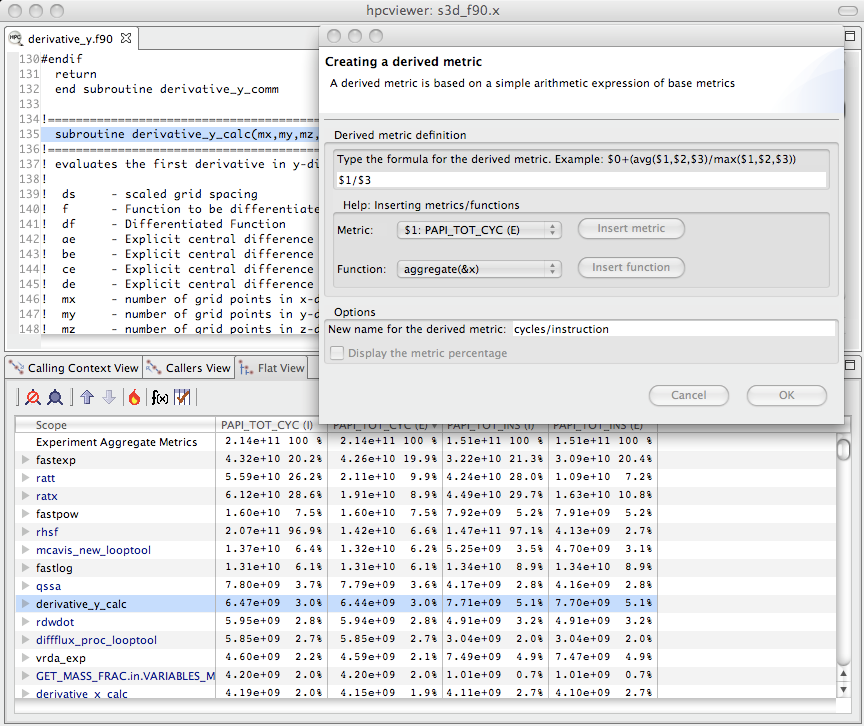
\includegraphics{figs/cycles-per-inst.png}}
%Two possible representations for the call path fragment $\ldots s_1 \rightarrow s_2 \ldots$, where $s_1$ and $s_2$ are call sites and where $s_1$ represents a call from $p$ to $q$ and $s_2$ a call from $q'$ to $r$.
\caption{Computing a derived metric (cycles per instruction) in {\tt hpcviewer}.}
\label{fig:cycles-per-inst}
\end{figure}

Figure~\ref{fig:cycles-per-inst} shows how to use {\tt hpcviewer} to compute a {\em cycles}/{\em instruction} derived metric from measured metrics {\tt PAPI\_TOT\_CYC}  and {\tt PAPI\_TOT\_INS}; these metrics correspond to {\em cycles} and {\em total instructions executed} measured with the PAPI hardware counter interface. To compute a derived metric, one first depresses the button marked $f(x)$ above the metric pane; that will cause the pane for computing a derived metric to appear. Next, one types in the formula for the metric of interest. When specifying a formula, existing columns of metric data are referred to using a positional name \$$n$ to refer to the $n^{th}$ column, where the first column is written as \$0. The metric pane shows the formula $\$1/\$3$. Here, \$1 refers to the column of data representing the exclusive value for {\tt PAPI\_TOT\_CYC} and \$3 refers to the column of data representing the exclusive value for {\tt PAPI\_TOT\_INS}.\footnote{An {\em exclusive} metric for a scope refers to the quantity of the metric measured for that scope alone; an {\em inclusive} metric for a scope represents the value measured for that scope as well as costs incurred by any functions it calls. In {\tt hpcviewer}, inclusive metric columns are marked with ``(I)'' and exclusive metric columns are marked with ``(E)." } Positional names for metrics you use in your formula can be determined using the {\em Metric} pull-down menu in the pane. If you select your metric of choice using the pull-down, you can insert its positional name into the formula using the {\em insert metric} button, or you can simply type the positional name directly into the formula. 

\begin{figure}[t]
\center{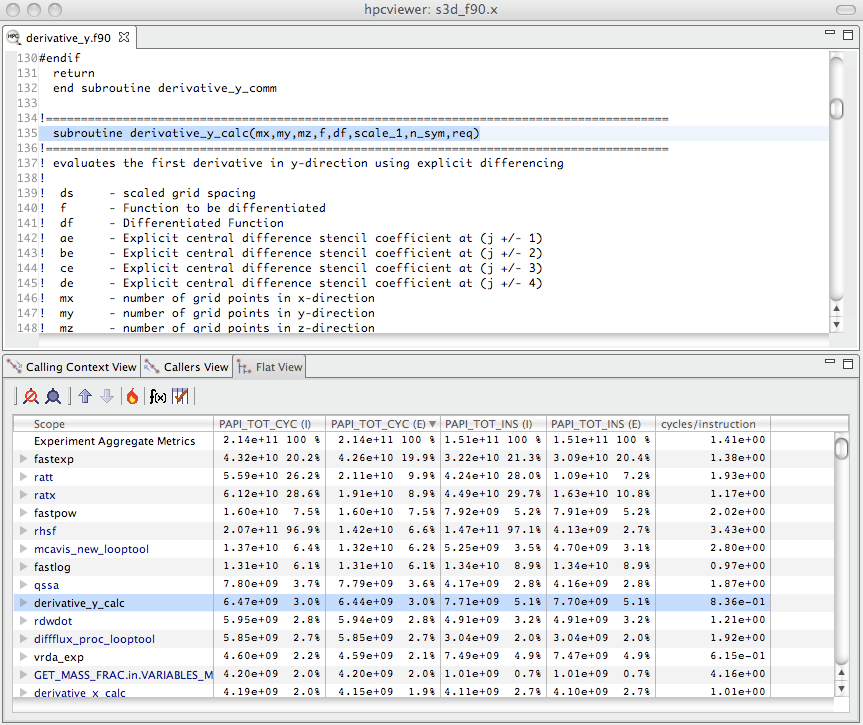
\includegraphics{figs/cycles-per-inst-2.png}}
%Two possible representations for the call path fragment $\ldots s_1 \rightarrow s_2 \ldots$, where $s_1$ and $s_2$ are call sites and where $s_1$ represents a call from $p$ to $q$ and $s_2$ a call from $q'$ to $r$.
\caption{Displaying the new {\em cycles/ instruction} derived metric  in {\tt hpcviewer}.}
\label{fig:cycles-per-inst-2}
\end{figure}

At the bottom of the derived metric pane, one can specify a name for the new metric. One also has the option to indicate that the derived metric column should report for each scope what percent of the total its quantity represents; for a metric that is a ratio, computing a percent of the total is not meaningful, so we leave the box unchecked. After clicking the OK button, the derived metric pane will disappear and the new metric will appear as the rightmost column in the metric pane. If the metric pane is already filled with other columns of metric, you may need to scroll right in the pane to see the new metric. Alternatively, you can use the metric checkbox pane (selected by depressing the button to the right of $f(x)$ above the metric pane) to hide some of the existing metrics so that there will be enough room on the screen to display the new metric. Figure~\ref{fig:cycles-per-inst-2} shows the resulting {\tt hpcviewer} display after clicking OK to add the derived metric.

The following sections describe several types of derived metrics that are of particular use to gain insight into performance bottlenecks and opportunities for tuning.

\section{Pinpointing and quantifying inefficiencies}

While knowing where a program spends most of its time or executes most of its floating point operations may be interesting, such information may not suffice to identify the biggest targets of opportunity for improving program performance. For program tuning, it is less important to know how much resources (\eg, time, instructions) were consumed in each program context than knowing where resources were consumed {\em inefficiently}.

To identify performance problems, it might initially seem appealing to compute ratios to see how many events per cycle occur in each program context. For instance, one might compute ratios such as FLOPs/cycle, instructions/cycle, or cache miss ratios. However, using such ratios as a sorting key to identify inefficient program contexts can misdirect a user's attention. There may be program contexts (\eg, loops) in which computation is terribly inefficient (\eg, with low operation counts per cycle); however, some or all of the least efficient contexts may not account for a significant amount of execution time. Just because a loop is inefficient doesn't mean that it is important for tuning. 

The best opportunities for tuning are where the aggregate performance losses are greatest. For instance, consider a program with two loops. 
The first loop might account for 90\% of the execution time and run at 50\% of peak performance. The second loop might account for 10\% of the execution time, but only achieve 12\% of peak performance. In this case, the total performance loss in the first loop accounts for 50\% of the first loop's execution time, which corresponds to 45\% of the total program execution time. The 88\% performance loss in the second loop would account for only 8.8\% of the program's execution time. In this case, tuning the first loop has a greater potential for improving the program performance even though the second loop is less efficient.

A good way to focus on inefficiency directly is with a derived {\em waste} metric.  Fortunately, it is easy to compute such useful metrics. However, there is no one {\em right} measure of waste for all codes. Depending upon what one expects as the rate-limiting resource (\eg, floating-point computation, 
memory bandwidth, etc.), one can define an appropriate waste metric (\eg, FLOP opportunities missed, bandwidth not consumed) and sort by that. 


\begin{figure}[t]
\center{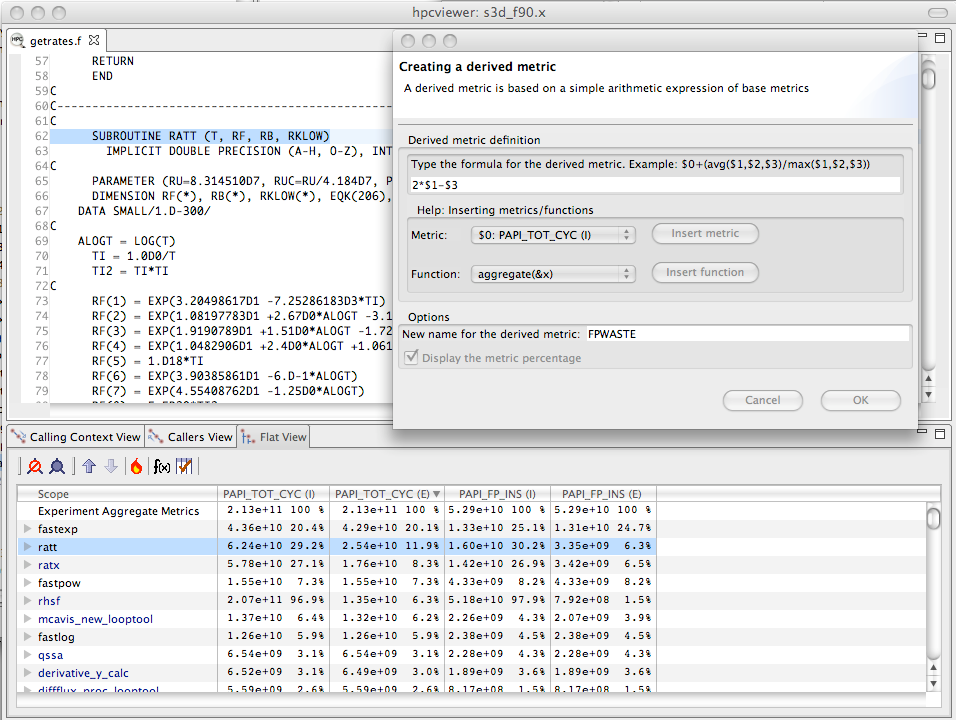
\includegraphics{figs/fpwaste.png}}
%Two possible representations for the call path fragment $\ldots s_1 \rightarrow s_2 \ldots$, where $s_1$ and $s_2$ are call sites and where $s_1$ represents a call from $p$ to $q$ and $s_2$ a call from $q'$ to $r$.
\caption{Computing a floating point waste metric in {\tt hpcviewer}.}
\label{fig:fpwaste}
\end{figure}

For instance, in a floating-point intensive code, one might consider keeping the floating point pipeline full as a metric of success. One can directly quantify and pinpoint losses from failing to keep the floating point pipeline full {\em regardless of why this occurs}. One can pinpoint and quantify losses of this nature by computing a {\em floating-point waste} metric that is calculated as the difference between the potential number of calculations that could have been performed if the computation was running at its peak rate minus the actual number that were performed.  To compute the number of calculations that could have been completed in each scope, multiply  the total number of cycles spent in the scope by the peak rate of operations per cycle. 
Using {\tt hpcviewer}, one can specify a formula to compute such a derived metric and it will compute the value of the derived metric for every scope. Figure~\ref{fig:fpwaste} shows the specification of this floating-point waste metric for a code.

Sorting by a waste metric will rank order scopes 
to show the scopes with the greatest waste. Such scopes correspond directly to those that contain the greatest opportunities for improving overall program performance. 
A waste metric will typically highlight loops where 
\begin{itemize}
\item a lot of time is spent computing efficiently, but the aggregate inefficiencies accumulate,
\item less time is spent computing, but the computation is rather inefficient, and
\item scopes such as copy loops that contain no computation at all, which represent a complete waste according to a metric such as floating point waste.
\end{itemize}

\begin{figure}[t]
\center{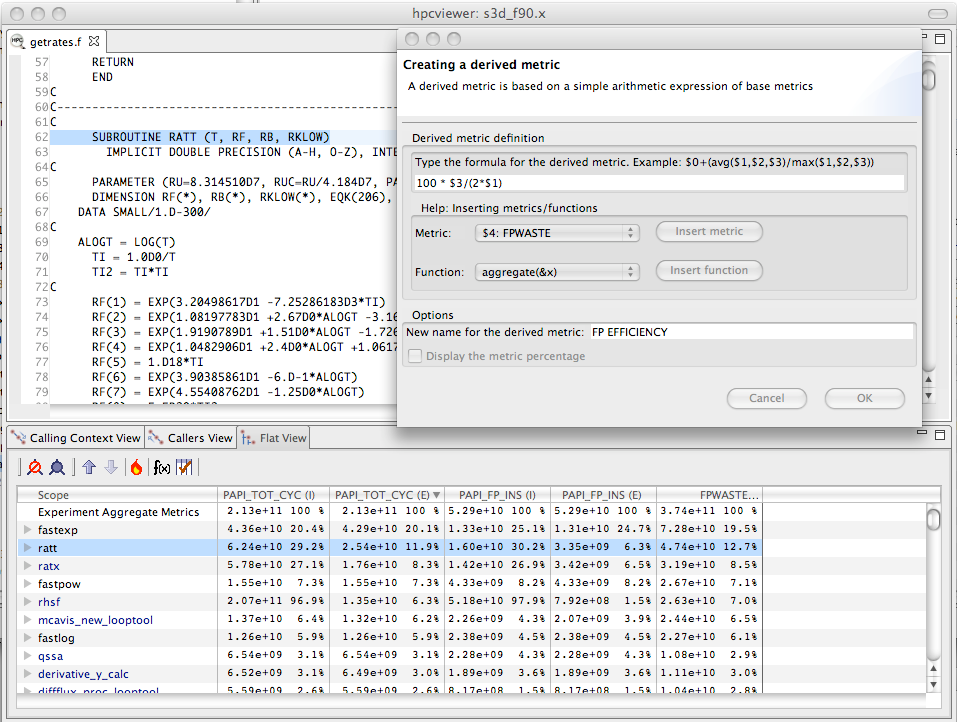
\includegraphics{figs/fp-efficiency.png}}
%Two possible representations for the call path fragment $\ldots s_1 \rightarrow s_2 \ldots$, where $s_1$ and $s_2$ are call sites and where $s_1$ represents a call from $p$ to $q$ and $s_2$ a call from $q'$ to $r$.
\caption{Computing floating point efficiency in percent using {\tt hpcviewer}.}
\label{fig:fpefficiency}
\end{figure}

Beyond identifying and quantifying opportunities for tuning with a waste metric, one can compute a companion 
derived metric {\em relative efficiency} metric to help understand how easy it might be to improve performance. 
A scope running  at very high efficiency will typically be much harder to tune than running at low efficiency.
For our floating-point waste metric, we one can compute the floating point efficiency metric by dividing measured FLOPs by 
potential peak FLOPS and multiplying the quantity by 100. Figure~\ref{fig:fpefficiency} shows the specification of this floating-point efficiency metric for a code.

\begin{figure}[t]
\center{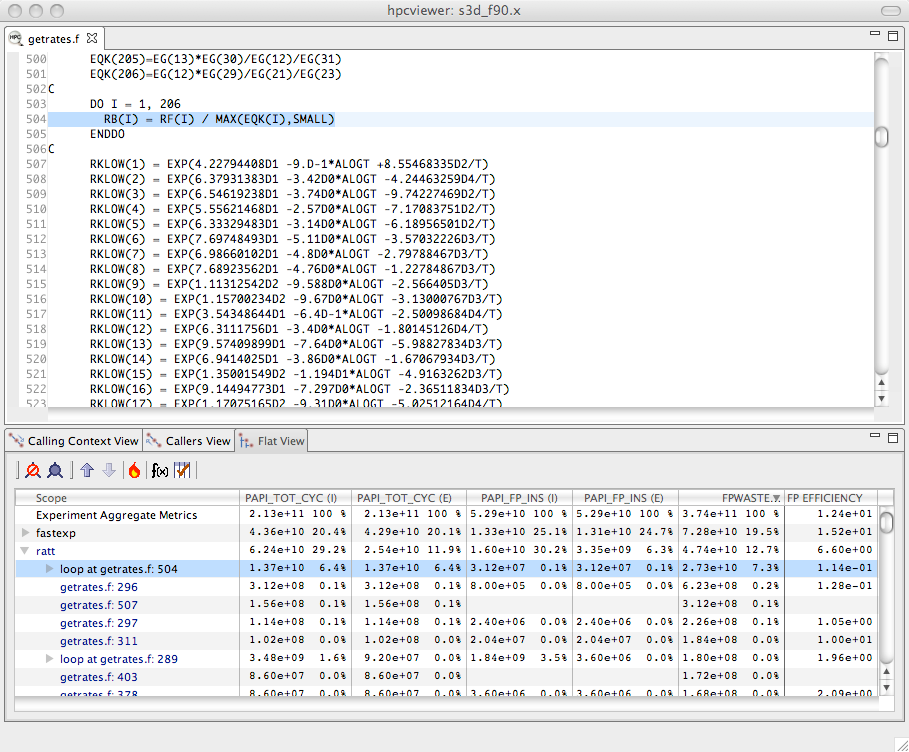
\includegraphics{figs/fp-efficiency-loop.png}}
%Two possible representations for the call path fragment $\ldots s_1 \rightarrow s_2 \ldots$, where $s_1$ and $s_2$ are call sites and where $s_1$ represents a call from $p$ to $q$ and $s_2$ a call from $q'$ to $r$.
\caption{Using floating point waste and the percent of floating point efficiency to evaluate opportunities for optimization.}
\label{fig:fpefficiency-loop}
\end{figure}

Scopes that rank high according to a waste metric and low according to a companion relative efficiency metric often make the best targets for optimization. Figure~\ref{fig:fpefficiency-loop} shows the specification of this floating-point efficiency metric for a code. Figure~\ref{fig:fpefficiency-loop} shows an {\tt hpcviewer} display that shows the top two routines that collectively account for 32.2\% of the floating point waste in a reactive turbulent combustion code. The second routine ({\tt ratt}) is expanded to show the loops and statements within. While the overall floating point efficiency for {\tt ratt} is at 6.6\% of peak (shown in scientific notation in the {\tt hpcviewer} display), the most costly loop in {\tt ratt} that accounts for 7.3\% of the floating point waste is executing at only .114\%.  Identifying such sources of inefficiency is the first step towards improving performance via tuning.

\section{Pinpointing and quantifying scalability bottlenecks}

On large-scale parallel systems,  identifying impediments to scalability is of paramount importance. On today's systems fashioned out of multicore processors, two kinds of scalability are of particular interest: 
\begin{itemize}
\item scaling within nodes, and
\item scaling across the entire system. 
\end{itemize}
\HPCToolkit{} can be used to readily pinpoint both kinds of bottlenecks. Using call path profiles collected by {\tt hpcrun}, it is possible to quantify and pinpoint scalability bottlenecks of any kind, {\em regardless of cause}.

To pinpoint scalability bottlenecks in parallel programs, we use {\em differential profiling}---mathematically combining corresponding buckets of two or more execution profiles. Differential profiling was first described by McKenney~\cite{mckenney98}; he used differential profiling to compare two {\em flat} execution profiles. Differencing of flat profiles is useful for identifying what parts of a program  incur different costs in two executions. Building upon McKenney's idea of differential profiling, we  compare call path profiles of parallel executions at different scales to pinpoint scalability bottlenecks. Differential analysis of call path profiles pinpoints not only differences  between two executions (in this case scalability losses), but the contexts in which those differences occur. Associating changes in cost with full calling contexts is particularly important for pinpointing context-dependent behavior. Context-dependent behavior is common in parallel programs. For instance, in message passing programs, the time spent by a call to {\tt MPI\_Wait} depends upon the context in which it is called. Similarly, how the performance of a communication event scales as the number of processors in a parallel execution increases depends upon a variety of factors such as whether the size of the data transferred increases and whether the communication is collective or not.

\subsection{Scalability analysis using expectations}
Application developers have expectations about how the performance of their code should scale as the number of processors in a parallel execution increases. Namely,
\begin{itemize}
\item when different numbers of
processors are used to solve the same problem (strong scaling), one
expects an execution's speedup to increase linearly with the number of processors employed;
\item when
different numbers of processors are used but the amount of computation
per processor is held constant (weak scaling), one expects the execution
time on a different number of processors to be the same.
\end{itemize}

In both of these situations, a code developer can express their expectations for how performance will scale as a formula that can be used to predict execution performance on a different number of processors. One's expectations about how overall application performance should scale can be applied to each context in a program
to pinpoint and quantify deviations from expected scaling. Specifically, one can scale and difference the performance of an application on different numbers of processors to pinpoint contexts that are not scaling ideally.

To pinpoint and quantify scalability bottlenecks in a parallel application, we first use {\tt hpcrun} to a collect call path profile for an application on two different numbers of processors.  Let $E_p$ be an execution on $p$ processors and $E_q$ be an execution on $q$ processors. Without loss of generality, assume that $q > p$.

In our analysis, we consider both {\it inclusive} and {\it exclusive}
costs for CCT nodes.  The inclusive cost at $n$ represents the sum of
all costs attributed to $n$ and any of its descendants in the CCT, and
is denoted by $I(n)$.  The exclusive cost at $n$ represents the sum of
all costs attributed strictly to $n$, and we denote it by $E(n)$. If
$n$ is an interior node in a CCT, it represents an invocation of a
procedure.  If $n$ is a leaf in a CCT, it represents a statement inside
some procedure. For leaves, their inclusive and exclusive costs are equal.

It is
useful to perform scalability analysis for both inclusive and
exclusive costs; if the loss of scalability attributed to the
inclusive costs of a function invocation is roughly equal to the loss
of scalability due to its exclusive costs, then we know that the
computation in that function invocation doesn't scale. However, if the
loss of scalability attributed to a function invocation's inclusive
costs outweighs the loss of scalability accounted for by exclusive
costs, we need to explore the scalability of the function's callees.



Given CCTs for an ensemble of executions, the next step to analyzing the scalability of their 
performance is to clearly define our
expectations. Next, we describe performance expectations for weak scaling and intuitive metrics that represent how much performance deviates from our expectations. More information about our scalability analysis technique can be found elsewhere~\cite{coarfa:ICS07}.

\begin{figure}[t]
\center{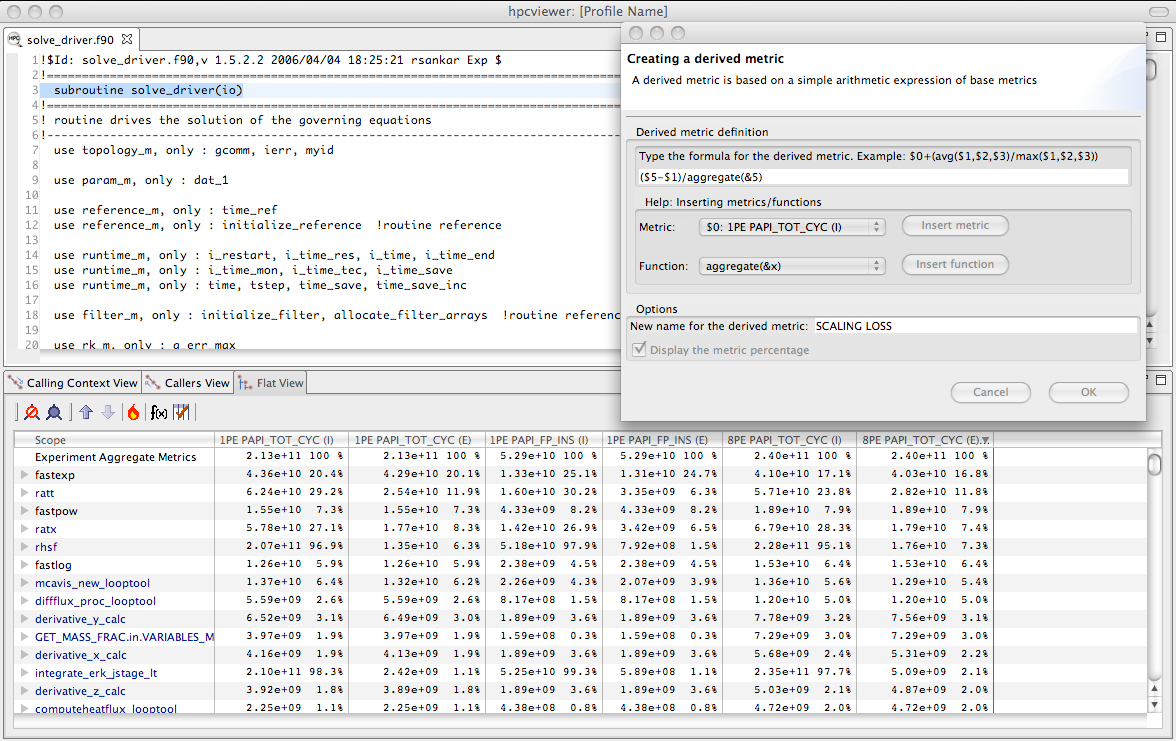
\includegraphics{figs/scaling-loss.png}}
%Two possible representations for the call path fragment $\ldots s_1 \rightarrow s_2 \ldots$, where $s_1$ and $s_2$ are call sites and where $s_1$ represents a call from $p$ to $q$ and $s_2$ a call from $q'$ to $r$.
\caption{Computing the fraction of excess work in each program scope when applying weak scaling to go from simulating a $30^3$ domain on one core to simulating a $60^3$ domain on eight cores of an AMD Barcelona. The fraction of excess work is a quantitative measure of scalability loss.}
\label{fig:scaling-loss}
\end{figure}

\begin{figure}[t]
\center{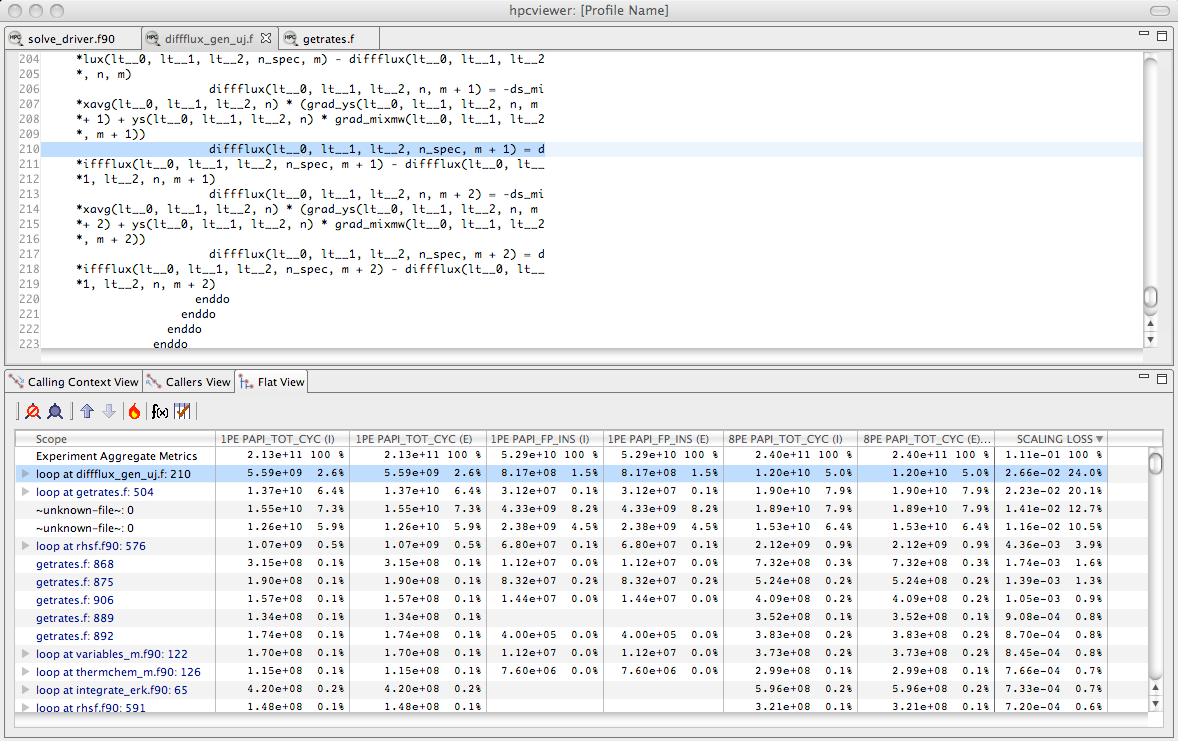
\includegraphics{figs/scaling-loss-2.png}}
%Two possible representations for the call path fragment $\ldots s_1 \rightarrow s_2 \ldots$, where $s_1$ and $s_2$ are call sites and where $s_1$ represents a call from $p$ to $q$ and $s_2$ a call from $q'$ to $r$.
\caption{Using the fraction the scalability loss metric of Figure~\ref{fig:scaling-loss} to rank order loop nests by their scaling loss.}
\label{fig:scaling-loss-2}
\end{figure}

\subsubsection*{Weak Scaling}

Consider two weak scaling experiments executed on $p$ and $q$ processors,
respectively, $p<q$. In Figure~\ref{fig:scaling-loss} shows how we can
use a derived metric to compute and attribute scalability losses. Here, we
compute the difference in exclusive cycles spent on one core of an 8-core
run and one core in a single core run in a weak scaling experiment. If the
code had perfect weak scaling, the time for the one core and the eight
core executions would be identical. We compute the fraction of excess
work by computing the difference for each scope between the time on the
eight core run minus the time on the single core run, and divide that by
the total time spent on the eight core run. This formula tells us how
much extra time we spent on the eight core run, attributes differences
to each scope. By normalizing by the total time spent in the eight core
run, we attribute to each scope the fraction of the total excess time in
the execution that was spent in that scope when scaling from one to eight
cores.\footnote{In {\tt hpcviewer}, we compute this metric for each scope
$s$ by subtracting the exclusive time spent in $s$ on one core (\$1) from
the time spent in $s$ on eight cores (\$5), and normalizing this quantity
by the aggregate total time spent on 8 cores ({\tt aggregate(\&5)}).}
This calculation pinpoints and quantifies scaling losses within a
multicore node. A similar analysis can be applied to compute scaling
losses between pairs of jobs scaled across an entire parallel system and
not just within a node. In  In Figure~\ref{fig:scaling-loss-2}, we rank
order loop nests by their scaling loss metric.  The source pane shows
the loop nest responsible for the greatest scaling loss when scaling
from one to eight cores. Unsurprisingly, the loop with the worst scaling
loss is very memory intensive. Memory bandwidth is a precious commodity
on multicore processors.

While we have shown how to compute and attribute the fraction of excess
work in a weak scaling experiment, one can compute a similar quantity
for experiments with strong scaling, except that the work on the larger
number of processors has to have a corrective multiplier applied to
account for the smaller fraction of work it receives.

\subsubsection{Exploring scaling losses}

Scaling losses can be explored in {\tt hpcviewer} using any of its three views.

\begin{itemize}
\item {\em Calling context view.} This top-down view represents the dynamic calling contexts (call paths) in which costs were incurred. 
\item {\em Callers view.}  This bottom up view enables one to look upward along call paths. This view is particularly useful for understanding the performance of software components or procedures that are used in more than one context, such as communication library routines.
\item {\em Flat view.} This view organizes performance measurement data according to the static structure of an application. All costs incurred in {\em any} calling context by a procedure are aggregated together in the flat view. 
\end{itemize}

\hpcviewer{} enables developers to explore top-down, bottom-up, and flat views
of  CCTs annotated with costs, helping to quickly pinpoint performance
bottlenecks. Typically, one begins analyzing an application's scalability
and performance using the top-down calling context tree view. Using this
view, one can readily see how costs and scalability losses are associated
with different calling contexts. If costs or scalability losses are
associated with only a few calling contexts, then this view suffices for
identifying the bottlenecks. When scalability losses are spread among many
calling contexts, \eg, among different invocations of {\tt MPI\_Wait},
often it is useful to switch to the bottom-up {\em caller's view} of
the data to see if many losses are due to the same underlying cause. In
the bottom-up view, one can sort routines by their exclusive scalability
losses and then look upward to see how these losses accumulate from the
different calling contexts in which the routine was invoked.

Scaling loss based on excess work is intuitive; perfect scaling
corresponds to a excess work value of $0$, sublinear scaling yields
positive values, and superlinear scaling yields negative values.
Typically, CCTs for SPMD programs have similar structure. If CCTs for
different executions diverge, using {\tt hpcviewer} to compute and report
excess work will highlight these program regions.

Inclusive excess work and exclusive excess work serve as useful measures
of scalability associated with nodes in a calling context tree (CCT).
By computing both metrics, one can determine whether the application
scales well or not at a CCT node and also pinpoint the cause of any lack
of scaling. If a node for a function in the CCT has comparable positive
values for both inclusive excess work and exclusive excess work, then the
loss of scaling is due to computation in the function itself.  However,
if the inclusive excess work for the function outweighs that accounted
for by its exclusive costs, then one should explore the scalability
of its callees.  To isolate code that is an impediment to scalable
performance, one can use the {\em hot path} button in {\tt hpcviewer}
to trace a path down through the CCT to see where the cost is incurred.


% ---------------------------------------------------------------------------
% ---------------------------------------------------------------------------
\clearpage
\bibliographystyle{abbrv}

\vspace{-18pt}
\bibliography{refs}

\end{document}

